\documentclass[12pt,preprint]{aastex}
\usepackage{url}
\usepackage{natbib}
\usepackage{graphicx}
%\usepackage{subfig}
%\usepackage{fixltx2e}

%%%%%%%%%%%%%%%%%%%%%%%%%%%%%%%%%%%%%%%%%%%%%%%%%%%%
%%% author-defined commands
\newcommand\x         {\hbox{$\times$}}
\def\mic              {\hbox{$\mu{\rm m}$}}
\def\about            {\hbox{$\sim$}}
\def\Mo               {\hbox{$M_{\odot}$}}
\def\Lo               {\hbox{$L_{\odot}$}}

%\captionsetup[figure]{labelformat=simple}
%%%%%%%%%%%%%%%%%%%%%%%%%%%%%%%%%%%%%%%%%%%%%%%%%%%%


\begin{document}

\title{Moving Object Pipeline Requirements}

\author{}

\begin{abstract}

The Moving Object Pipeline System (MOPS) is responsible for generating
and managing the \textbf{Moving Object} data products.  The Moving
Objects are identified solar system objects (SSOs) with associated
Keplerian orbits, errors, and a detected sources assocated with those
solar system objects.  The Moving Object database will also be used by
the Association Pipeline to future locations of moving objects in
incoming images, preventing the generation of Alerts on detections of
known Solar System objects.  We present the relationship of the MOPS
to overall LSST Data Management and provide a brief overview of the
methods used within the MOPS.

\end{abstract}

\tableofcontents

%\section{Science Requirements}

\section{System Design and Responsibilities}

 
% ILLUSTRATIONS: DayMOPS, NightMOPS, MovingObjects database, telescope control

\begin{figure}[!ht]
\begin{center}
  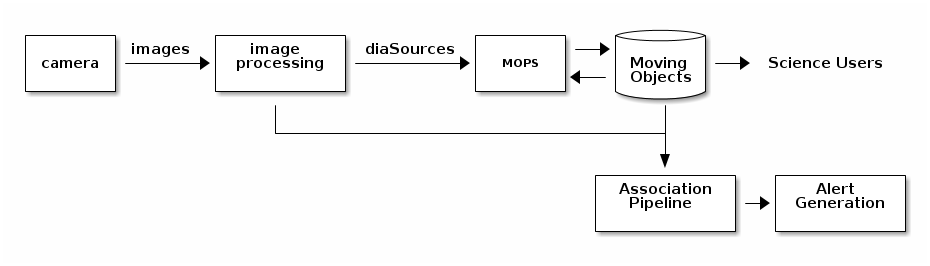
\includegraphics[width=13cm]{illustrations/mopsWithinLsst.png}
\end{center}
\caption{The Moving Object Pipeline System uses transient detections
  (diaSources) discovered by the image processing pipeline to generate
  and update the Moving Object table. }
\end{figure}


The Moving Object Pipeline System (MOPS) is responsible for
discovering new Moving Objects in newly-acquired data, searching old
data for detections of new objects, and updating the Moving Objects
table to reflect newly-acquired data. It is also responsible for
periodically cleaning and refining the contents of the Moving Objects
table.


\subsection{Discovering and Managing Moving Objects}


The initial task of DayMOPS is to identify unknown objects present in
images and their orbits.  To accomplish this, the system initially
finds sets of detections which follow a sky-plane path roughly
consistent with asteroid motion; these sets of detections and their
fitted paths are called \textbf{tracks}.  This same method is the
basis for asteroid discovery used in the PanSTARRS Moving Object
Pipeline System \citep{psMOPSDesign}.  A set of algorithms for the
discovery of sky-plane tracks in dense data are presented in
\citet{Kubica:2005:MTA:1081870.1081889}; these algorithms are used in
the PanSTARRS MOPS as well.  Because of the loose approximations used,
many of the tracks will be mislinkages, combining detections which are
not attributable to the same source, but virtually all objects for
which a true (correctly-linked) track could be generated will get some
correct track.  LSST Data Management has developed additional
processing phases and filters which can improve the performance of the
system and reduce the computational costs by managing the number of
untrue or redundant tracks throughout the various phases of
processing.

% possible paragraph on limitations: discuss the one-month cutoff, the
% tracklets, the revisit rate issues

Once tracks are discovered, they are sent to the Orbit Determination
phase. The Orbit Determination phase takes these sets of sky-plane
detections and attempts to find a Kepler orbit which could generate
the detections, if any exists.  This orbit is further refined, and
error bounds are established, using least-squares linearization.
Orbit Determination will reject many tracks as false, but should
successfully find fairly precise orbits for virtually all correctly
linked tracks.  Several methods for performing this task are known,
and several have implementations available to LSST
\citep{Milani04orbitdetermination}, \citep{Milani2006},
\citep{OpenOrb2009}, \citep{granvik_thesis}.  These orbits, and the
detections present in the track associated with that orbit, are used
to generate new Moving Objects.

\begin{figure}[h]
\begin{center}
  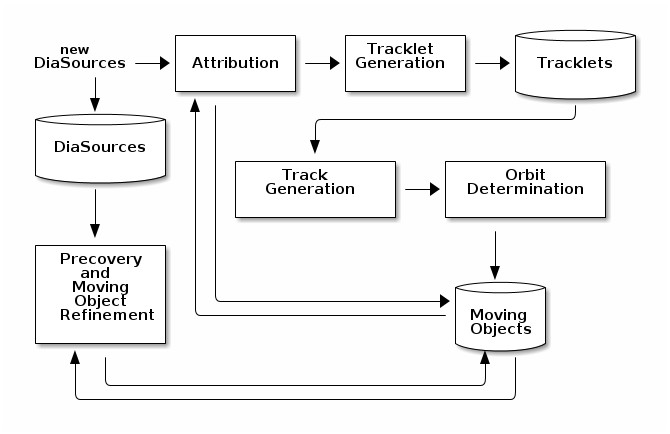
\includegraphics[width=11cm]{illustrations/mopsDiagram.png}
\end{center}
\caption{ Input detections (diaSources) sent to the MOPS are processed
  through a multi-stage pipeline to generate the eventual Moving
  Objects.} 
\end{figure}


As in the PanSTARRS MOPS design \citep{psMOPSDesign} the LSST's MOPS
is expected to perform several additional tasks to manage and improve
the Moving Objects table over time.  Attribution is the process of
identifying known objects in incoming data and adding those detections
to the correct Moving Object (this task is delegated to
NightMOPS). Precovery is another task, the recovery of known,
unattributed detections associated with a newly-discovered Moving
Object.  Another refinement is the merging of potentially redundant
Moving Objects.


\subsection{NightMOPS: Predicting Moving Object Locations}

The NightMOPS section of MOPS is responsible for predicting the
locations of known Moving Objects as images are taken, so that they
may be attributed to the known Moving Objects and removed from the set
of unknown transients detections.  This allows attribution for known
Moving Objects, improving the quality of the Moving Object data
products, and also allows the prevention of unnecessary Alerts.

Predicting the locations of objects given an orbit can be accomplished
through ephemeris calculation using existing orbit-space software
suites \citep{Milani2006}, \citep{OpenOrb2009}.  However, ephemeris
calculation can be fairly slow due for large data sets.  Because the
observations schedule for LSST will be determined dynamically, it is
necessary to generate ephemeris predictions for a large Moving Object
table in a short period of time.

% some kind of time-domain illustration?

In order to accomplish this, NightMOPS will generate ``coarse
ephemerides'' for known objects, predicting their locations at the
beginning and end of the night.  Then, when given an upcoming image
location, NightMOPS will use interpolation of the coarse ephemerides
to find objects which could feasibly be present in the upcoming
image. Precise ephemerides for just these objects will be
generated. In this way, NightMOPS will avoid the problem of generating
ephemeris for each known Moving Object for every image time.


\subsection{Implementation Status}

All software components of MOPS, with the possible exception of
initial orbit determination, and orbital least-squares linearization
fitting of orbits to data, and ephemeris generation, is expected to be
completed in open-source C++ compliant with LSST software guidelines
and in LSST appropriate coding style.  These components will run
inside the LSST Pipeline Framework.  

Currently, the initial tracking phases of DayMOPS are implemented in
LSST-compliant C++.  The selection of an appropriate package for
initial orbit determination, least-squares linearization of orbit
fitting, and ephemeris generation is incomplete but several FORTRAN
options are available to us, some open-source.  A Python-based
implementation of NightMOPS, using the LSST Pipeline Framework, is
complete but it is currently using a closed-source ephemeris
generation tool.




\section{MOPS Metrics \& Scaling}



\section{Development Plan}



\bibliographystyle{apj}
\bibliography{baseline}

\end{document}
